\section{Definitions}\label{sect:definitions}
Although theoretical examination is not central to this work, the interested
reader shall be introduced to the most fundamental concepts in this section.

Namely
\begin{enumerate*}[a.)]
    \item what is the data structure (time series),
    \item what are we trying to retrieve (anomalies), and
    \item how are we retrieving it (anomaly detection).
\end{enumerate*}

\subsection{What is the data structure?}
System-health data is produced in a variety of formats. Most commonly it comprises
multiple simultaneously produced streams of either natural language (in form of
log-messages~\cite{Zietlow.2020}) or numerical data.

To reduce complexity, only univariate streams of numerical data will be considered
in this paper.

\begin{definition}[Observation]
    Observations are numerical values observed at a certain point in time.
    Mathematically, it is the tuple given in \cref{eq:observation}
    
    \begin{equation}\label{eq:observation}
        \text{Observation}\ o := (t, y)
    \end{equation}
    where:
    \begin{conditions}
        \text{timestamp } t & \in{} & \(\mathbb{Z}\)\\
        \text{value } y      & \in{} & \(\mathbb{R}\)
    \end{conditions}
    
    The timestamp can be further interpreted as unix epoch time, coarsely given in \cref{eq:unix-time}
    \begin{equation}\label{eq:unix-time}
        \begin{cases}
            \text{before 01 Jan 1970 00:00:00 GMT},& {\text{if } t < 0}\\
            \text{01 Jan 1970 00:00:00 GMT},& {\text{if } t = 0}\\
            \text{after 01 Jan 1970 00:00:00 GMT},& {\text{if } t > 0}
        \end{cases}
    \end{equation}
\end{definition}

\begin{definition}[Time Series]\label{defn:time-series}
    A time series is the ordered set of multiple related observations.
    It can be indexed in two complementary ways, using either
    \begin{enumerate*}[a.)]
        \item the timestamp of the current observation \cref{eq:time-series-timestamp} or
        \item the count of the current observation \cref{eq:time-series-count}.
    \end{enumerate*}


    \begin{align}
        \text{Timestamp-Indexed TS}&:= \left\{ y^{(t_0)},\ldots, y^{\left(t_{T-1}\right)} \right\}\label{eq:time-series-timestamp}\\
        \text{Count-Indexed TS}&:= \left\{ o^{(0)},\ldots, o^{(T-1)} \right\}\label{eq:time-series-count}
    \end{align}
    where:
    \begin{conditions}
        T &:= & Number of observations\\
        t_i &:= & Timestamp of ith Observation\\
        o^{(i)} &:= & The ith observation\\
        y^{(t_i)} &:= & Value of the observation with timestamp \(t_i\)
    \end{conditions}

    From a practical standpoint, count-indexed time series are useful for e.g.\
    construction of sliding-windows or neighborhoods (\cref{def:neighborhood}),
    while timestamp-indexed time series are useful for e.g.\ inference of
    cyclicity (\cref{def:cyclicity})
\end{definition}

For system-health data time series, the observation \(o_t\) is usually
related to multiple other observations. Most obviously, \(o_t\) is related to 
values from its neighborhood (\cref{def:neighborhood}). Furthermore, it might
be influenced by multiple levels of cyclicity (\cref{def:cyclicity}).

\begin{definition}[Neighborhood]\label{def:neighborhood}
    The neighborhood of an observation in a time series is the set of its
    \(n\)-surrounding values. Mathematically given in \cref{eq:neighborhood}.

    \begin{equation}\label{eq:neighborhood}
        \left\{ o_{t-n/2},\ldots,o_{t+n/2} \right\} \setminus o_t,\ n\in \mathbb{N}
    \end{equation}
\end{definition}

\begin{definition}[Cyclicity]\label{def:cyclicity}
    A time series has some kind of cyclicity if it contains a pattern that repeats
    approximately every \(P\) steps, where \(P\) can be some random variable. In
    simple terms the time series TS is said to be (additively-constant) cyclic
    if \(\text{TS}(i + P) \approx \text{TS}(i) + C,\ C\in \mathbb{R}\). This
    definition could easily be extended to more complex cyclic patterns. For
    detailed examination see~\cite{Falk.2012}.
\end{definition}

\subsection{What are we trying to retrieve?}
Breakages can manifest visually in different forms. Common forms are
\begin{enumerate}
    \item\label{itm:1} a drop/peak significantly below/above previously observed values,
    \item\label{itm:2} a drop/peak below/above typical values of the neighborhood
    \item\label{itm:3} a drop/peak below/above its expected cyclic dependencies,
    \item\label{itm:4} a change point (lasting violation of a cyclic pattern).
\end{enumerate}
An influential taxonomy of such breakages has been introduced by \textcite{Chandola.2009}
as follows:

\begin{definition}[Point Anomaly]\label{def:point-anomaly}
    Point Anomalies are \textbf{singular} observation that deviate significantly
    from the general distribution~\cite[cf.][]{Chandola.2009}. This comprises
    common breakage form~\labelcref{itm:1}. A visualization is given in
    \cref{fig:point-anomaly}.
\end{definition}

\begin{definition}[Contextual Anomaly]\label{def:contextual-anomaly}
    Contextual Anomalies are \textbf{singular} observations which do not deviate
    strongly from the general distribution but only from its neighborhood or
    cyclic dependencies~\cite[cf.][]{Chandola.2009}. This comprises common breakage
    forms \labelcref{itm:2,itm:3}. A visualization is given in
    \cref{fig:contextual-anomaly}.
\end{definition}
 
\begin{definition}[Collective Anomaly]\label{def:collective-anomaly}
    Collective Anomalies are multiple data points which, in isolation, do not appear
    anomalous. When observed as a group however, they show unusual
    characteristics~\cite[cf.][]{Chandola.2009}. This comprises common breakage
    forms \labelcref{itm:3,itm:4}. A visualization is given in
    \cref{fig:collective-anomaly}.
\end{definition}

\begin{figure}[htp!]
    \begin{subfigure}[b]{.45\linewidth}
        \centering
        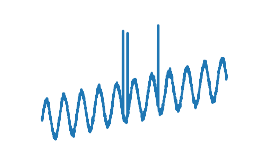
\includegraphics[width=.6\textwidth]{point_anomalies_yahoo!s5.png}
        \subcaption{Point anomalies from Yahoo!S5: A2Benchmark.synthetic\_11}\label{fig:point-anomaly}
    \end{subfigure}%
    \hfill
    \begin{subfigure}[b]{.45\linewidth}
        \centering
        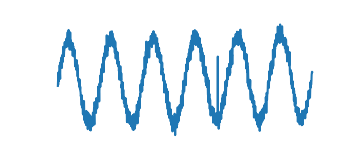
\includegraphics[width=.7\textwidth]{contextual_anomalies_yahoo!s5.png}
        \subcaption{Contextual anomaly from Yahoo!S5: A2Benchmark.synthetic\_15}\label{fig:contextual-anomaly}
    \end{subfigure}\\[1ex]
    \begin{subfigure}[b]{\linewidth}
        \centering
        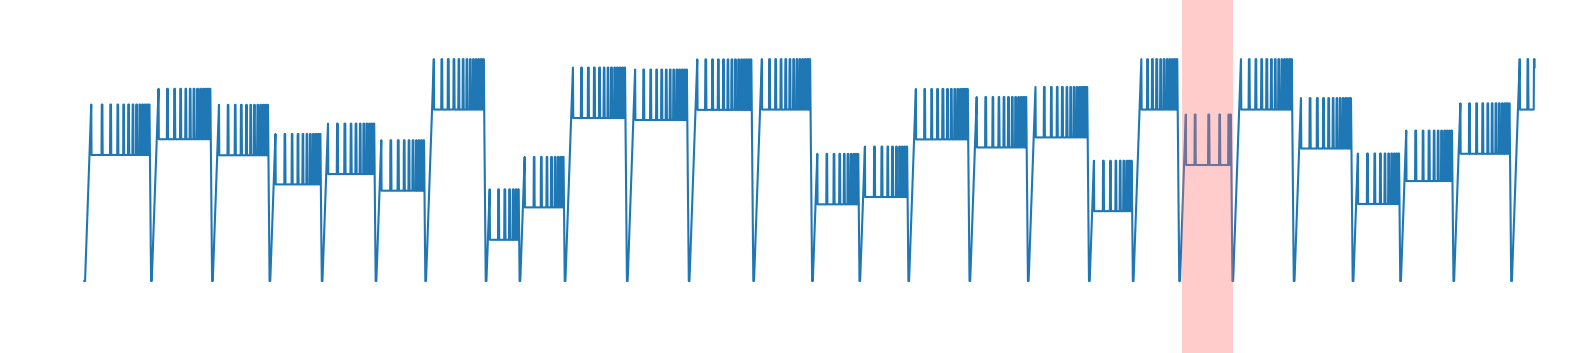
\includegraphics[width=\textwidth]{collective_anomaly_LevcorrTempfaultseed199vars23.RT_level.jpg}
        \subcaption{Collective anomalies from Gasoil-Dataset~\cite{Filonov.2016}: 48\_Lev\_corr\_Temp\_fault\_seed\_199\_vars\_23[``RT\_level''].}\label{fig:collective-anomaly}
    \end{subfigure}
    \caption{Illustration of the three anomaly types~\cite{Chandola.2009} from different datasets.}\label{fig:anomaly-types}
\end{figure}

All common breakage forms are included in one of the three anomaly definitions.
We therefore try to retrieve all data points which fall under one of the
\cref{def:point-anomaly,def:contextual-anomaly,def:collective-anomaly}.


\subsection{How are we retrieving it?}
Retrieval of anomalies as defined in \cref{def:point-anomaly,def:contextual-anomaly,def:collective-anomaly}
can be done via different paradigms. Extensive taxonomies have been proposed in~\cite{Chandola.2009,Zietlow.2020}.
Because theoretical examination is not central to this paper, the taxonomy will
be presented merely simplified and condensed.

Two major groups of algorithms can be considered: either Forecasting- or
Boundary-based:
\begin{definition}[Forecasting-Based]
    Forecasting-based algorithms consist of two major phases:
    \begin{enumerate}[a.)]
        \item In the first phase, the algorithm tries to predict the next \(n\)-observation
        given a learning history of previous observations. A predicted observation
        is denoted \(\hat{o}\). Deviations from the ground truth are recorded.
        A common approach would be to calculate the squared error \(e = {\left(o - \hat{o}\right)}^2\).
        \item In the second phase the current-error \(e\) is put in context with
        previously recorded error-terms. This is often done via 
        parametric~\cite{Malhotra.2015,Ahmad.2017,Guo.2016,Malhotra.2016,Shipmon.2017,Chauhan.2015} or 
        non-parametric statistical tests~\cite{Zhu.2017,Hundman.2018,Maimo.2018,Su.2019}.
        For details confer~\cite{Zietlow.2020}.
    \end{enumerate}
\end{definition}

\begin{definition}[Boundary-Based]
    Boundary-Based algorithms consist of only a single major phase:
    they try to calculate some boundary to which most observations conform.
    Observations beyond that boundary are deemed anomalous.
\end{definition}
